\chapter{Komunikacja}\label{ch:komunikacja} % Bardzo możliwe że nazwa do zmiany

Komunikacja odbywa się między robotem i drugim urządzeniem za pośrednictwem przewodu usb.
Raspberry pi w tym przypadku emuluje urządzenie szeregowe.
Dzięki temu łatwo jest podłączyć i korzystać z robota na większości systemów operacyjnych. 
Do obsługi komunikacji wykorzystywany jest skrypt wykonany w pythonie, który jest uruchamiany 
przez systemd po podłączeniu robota. Po uruchomieniu robot czeka na komendę która wybierze jego tryb pracy. 
% https://www.kernel.org/doc/Documentation/usb/gadget_serial.txt

\section{Tryb pracy} 

\subsection{Ciągłe generowanie danych}
Aby wykorzystać ten tryb pracy należy wysłać do robota przez port szeregowy znak 'e'.
W tym trybie zadaniem jest ciągłe generowanie kolejnych bajtów danych.
Odbywa się to przez wykonanie następującego algorytmu:\\
1. Wykonanie rzutu kością \\
2. Wykorzystanie modelu opisanego w~\ref{ch:odczytywanie-losowego-wyniku-z-kosci} do oczytania liczby i zapisanie jej do zmiennej a \\
3. Przesunięci bitowe zmiennej a w lewo o 3 bity \\
4. Powtórzenie kroku 1, 2 i 3 aż do wygenerowania co najmniej 8 bitów \\
5. Wydobycie bajtu ze zmiennej a i wysłanie go \\

W powyższym algorytmie dane wysyłane są po bajcie danych ponieważ dane w pamięci 
są wyrównane do bajtów więc jest najmniejszą jednostką, którą można przekazać na raz.
Głównym założeniem tego trybu pracy jest wykorzystanie go jako dodatkowe źródło entropii w systemie Linux, 
dla zobrazowania tego wykonany został diagram~\ref{fig:interface_a}.

\begin{figure}[H]
    \centering
    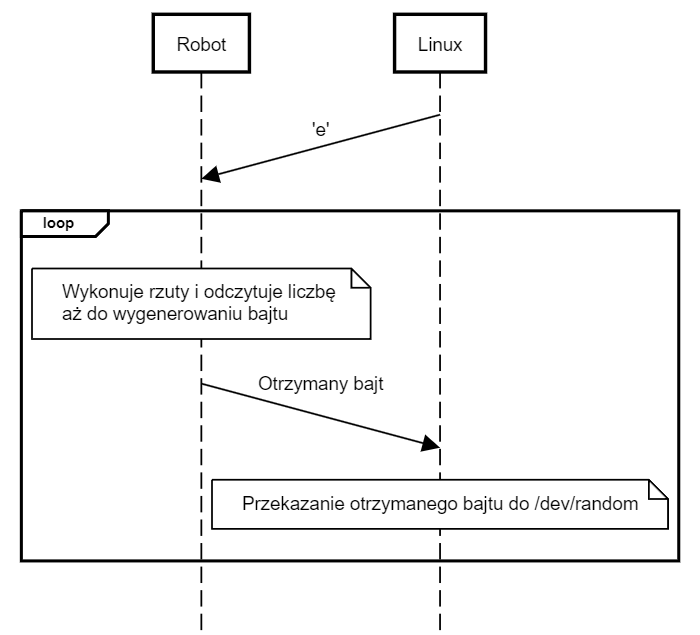
\includegraphics[width=0.5\linewidth]{chapters/05-Przetwarzanie Wyniku/figures/InterfaceA}
    \caption{Diagram sekwencji dla ciągłego generowania danych}
    \label{fig:interface_a}
\end{figure}

\subsection{Wykonywanie pojedyńczych rzutów}
Aby wykorzystać ten tryb pracy należy wysłać do robota przez port szeregowy znak 'd'.
W tym trybie zadaniem jest oczekiwanie na polecenie wykonania rzutu, czyli znak 'r'.
Kolejnie wykonanie rzutu kością i odpowiedź otrzymaną liczbą. Następnie otrzymaną liczbę można wykorzystać w swoim programie. Działanie to zobrazowano na diagramie~\ref{fig:interface_b}.

\begin{figure}[H]
    \centering
    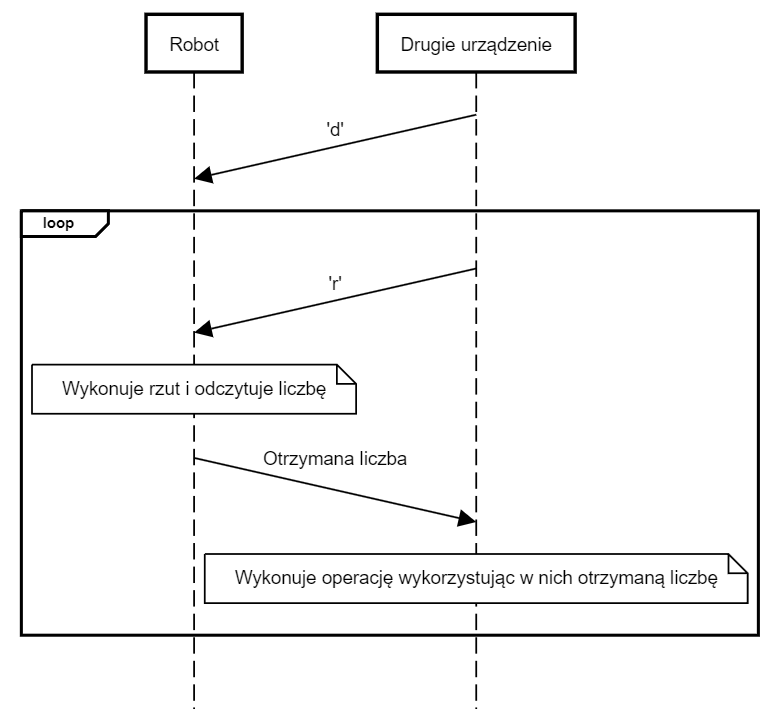
\includegraphics[width=0.5\linewidth]{chapters/05-Przetwarzanie Wyniku/figures/InterfaceB}
    \caption{Diagram sekwencji dla wykonania rzutu na żądanie}
    \label{fig:interface_b}
\end{figure}

